% This is samplepaper.tex, a sample chapter demonstrating the
% LLNCS macro package for Springer Computer Science proceedings;
% Version 2.21 of 2022/01/12
%
\documentclass[runningheads]{llncs}
%
\usepackage[T1]{fontenc}
% T1 fonts will be used to generate the final print and online PDFs,
% so please use T1 fonts in your manuscript whenever possible.
% Other font encondings may result in incorrect characters.
%
\usepackage{graphicx}
% Used for displaying a sample figure. If possible, figure files should
% be included in EPS format.
%
% If you use the hyperref package, please uncomment the following two lines
% to display URLs in blue roman font according to Springer's eBook style:
%\usepackage{color}
%\renewcommand\UrlFont{\color{blue}\rmfamily}
%\urlstyle{rm}
%
\usepackage{subcaption}

\begin{document}
%
\title{TheoremView: A Framework for Extracting Theorem-like Environments from Raw PDFs}
%
%\titlerunning{Abbreviated paper title}
% If the paper title is too long for the running head, you can set
% an abbreviated paper title here
%
\author{Shrey Mishra\inst{1}\orcidID{0000-0000-0000-0000} \and
Neil Sharma\inst{2}\orcidID{0000-0000-0000-0000} \and
Antoine Gauquier\inst{1}\orcidID{0009-0005-9573-6364} \and
Pierre Senellart\inst{1,3}\orcidID{0000-0002-7909-5369}}

\authorrunning{S. Mishra et al.}
% First names are abbreviated in the running head.
% If there are more than two authors, 'et al.' is used.

\institute{DI ENS, ENS, CNRS, PSL University, Inria, Paris, France \\
\email{shrey.mishra@ens.psl.eu, antoine.gauquier@ens.psl.eu, pierre@senellart.com}
\and
Malaviya National Institute of Technology \\
\email{neil.sharma3000@gmail.com}
\and
Institut Universitaire de France (IUF)
}

\maketitle              % typeset the header of the contribution
%
\begin{abstract}
This paper presents TheoremView, a novel modular multimodal framework designed 
to extract proofs and theorems from scientific papers in their raw PDF format, 
without requiring access to \LaTeX~source files. Our approach leverages three 
distinct modalities (font, text, and vision) to accurately identify and classify 
proof and theorem-like environments. We incorporate a sequential component to capture 
long-term dependencies, including page breaks and layout information. 
TheoremView employs a combination of specialized models trained to recognize 
and extract these critical elements from academic documents. By eliminating 
the need for OCR preprocessing, our method significantly reduces computational 
overhead, making it feasible for real-time applications. This innovative 
approach offers a robust solution for automated theorem extraction, potentially 
enhancing accessibility and analysis of mathematical content in scientific 
literature.

\keywords{Theorem extraction \and Multimodal learning \and Document analysis \and Machine learning \and Natural language processing}
\end{abstract}
%
%
%
\section{Introduction}
\subsection{Motivation for Theorem Extraction}
In contemporary scientific research, articles are primarily published as PDFs, and many 
search engines index entire papers instead of specific scientific results. This paper 
contributes to TheoremKB ~\cite{doceng_paper}, a project focused on building a knowledge base of mathematical 
results across different fields of science. The objective is to improve the accessibility of 
relevant information for researchers, allowing for more effective retrieval and utilization 
of scientific knowledge.

Having such a knowledge base can significantly impact the way researchers find information~\cite{mishra2024first}. 
Some advantages of this system include:

\begin{enumerate}
    \item \textbf{Enhanced Accessibility}: TheoremKB streamlines the retrieval of specific 
    proofs and theorems, allowing for quick access to targeted mathematical results, 
    in contrast to traditional search engines that index full-text papers.

    \item \textbf{Facilitated Knowledge Discovery}: This knowledge base assists researchers 
    in uncovering connections between disparate mathematical results and their applications, 
    thereby enhancing the exploration of specific results, such as NP-hardness in relation to 
    the vertex cover problem.

    \item \textbf{Identification of Theorem Interdependencies}: TheoremKB helps determine 
    which theorems are used in the proofs of others, which is essential for assessing the 
    impact of errors in foundational results.

    \item \textbf{Support for Automated Reasoning}: The knowledge base provides a foundation 
    for developing AI systems capable of automated theorem proving, promoting innovative 
    approaches to mathematical problem-solving.
\end{enumerate}

\subsection{Prior work on Theorems and Proofs Extraction}

Previous attempts to address this task include the work presented in~\cite{doceng_paper}, which focused on 
initial explorations of extraction from PDFs framed as object detection and text classification problems. 
This approach utilized font visuals and text modalities but operated only at the text-line level. Subsequent 
research, such as~\cite{jcdl_paper}, refined the methodology by incorporating contextual information 
surrounding paragraphs and employing multimodal systems to unify the extraction model.

The TheoremView framework offers a user interface to visualize the results extracted by various models in 
an end-to-end system that directly takes PDFs as input and displays the extracted results. It is designed 
modularly, allowing users to select which model to utilize for extraction, thereby leveraging different 
modalities that highlight the strengths and weaknesses of each approach. This flexibility enables users 
to run models on low-compute hardware, such as systems without GPU instances, for inference. The primary 
objective of this paper is to present an easy-to-use interface that facilitates preprocessing and inference 
in a modular manner.

\section{Methodology}
We propose a modular approach to extract raw information from PDFs. We utilize Grobid~\cite{GROBID} and pdfalto~\cite{pdfalto} to convert 
the documents into valid XML formats. The XML generated by Grobid organizes the content into paragraphs, 
while the XML from pdfalto provides details segmented into text lines along with associated font information. 
We then employ a merging script to correlate the font information with each paragraph extracted by Grobid. 
This process yields a CSV file structured by paragraphs, where each row includes the spatial location of the 
paragraph on the page (indicating page number, and both vertical and horizontal coordinates), the textual content 
extracted from Grobid, and the font information used within those paragraphs. For a schematic diagram on data pipeline
refer to figure \ref{fig:datapipeline}.

Importantly, we do not rely on any OCR preprocessing; instead, we leverage PDFALTO and Grobid, which are 
specialized tools that efficiently extract information from scientific articles. It is crucial to note that 
while we do not use \LaTeX~sources during inference, they are utilized solely for generating ground truths 
during model training.

\begin{figure}[h]
    \centering
    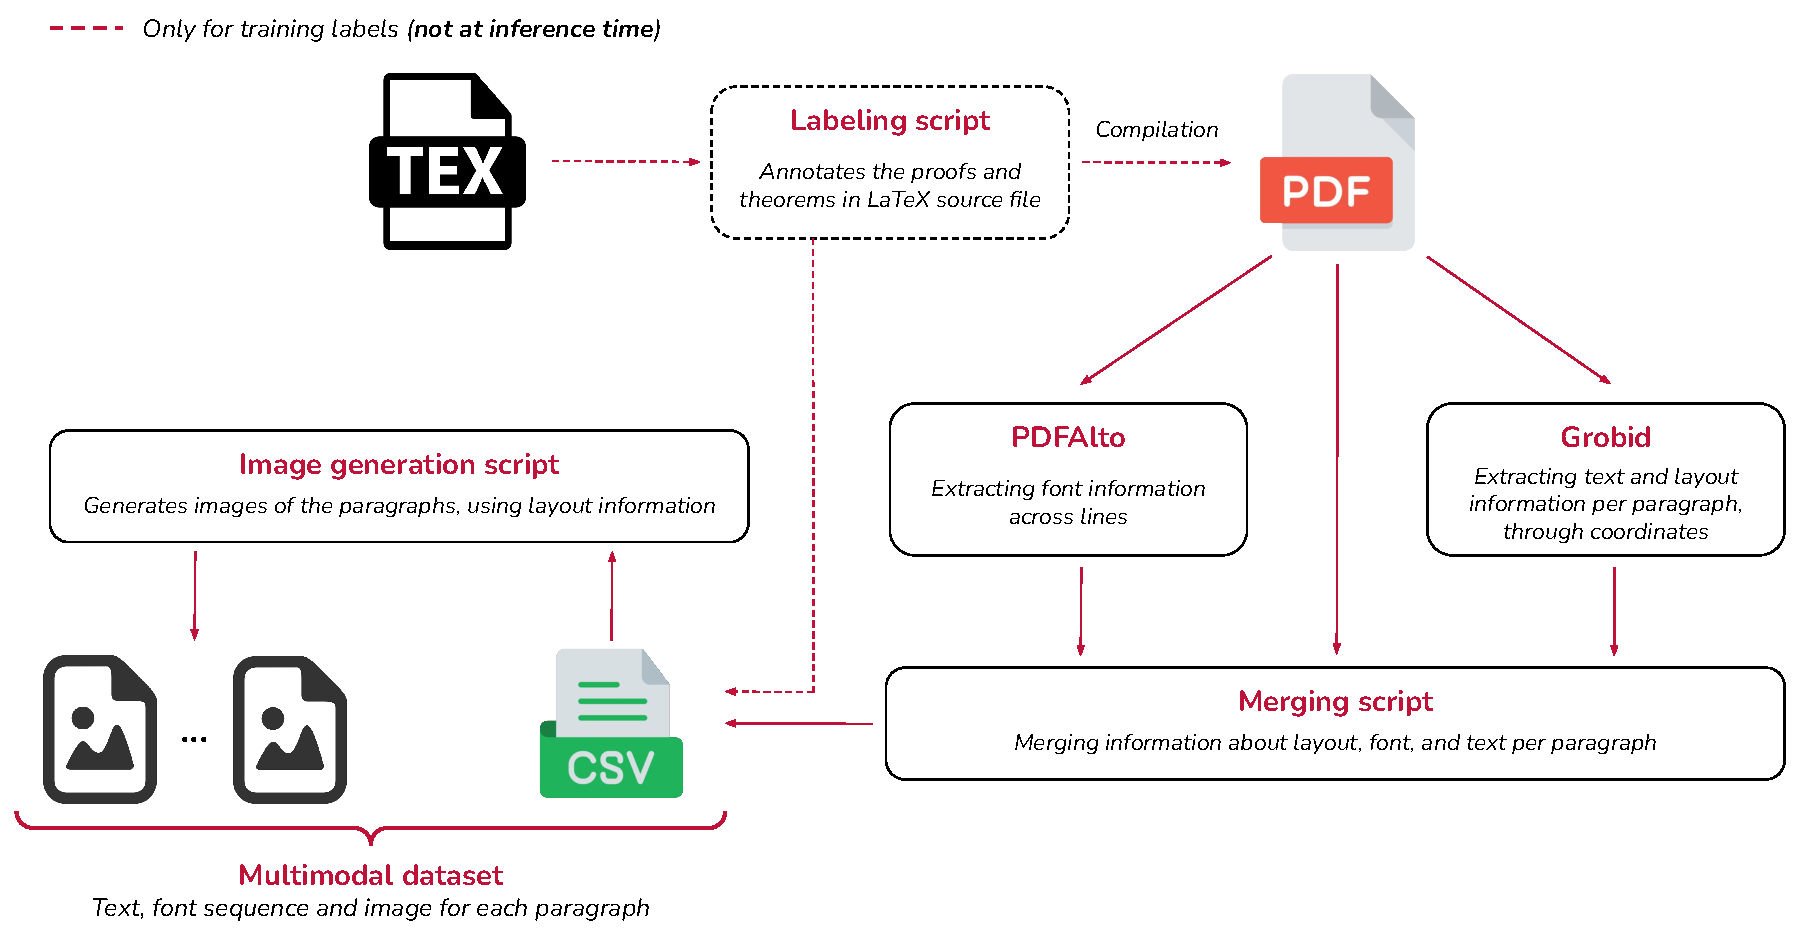
\includegraphics[width=\textwidth]{images/preprocessing.pdf}
    \caption{Data pipeline for extracting and processing information from PDFs.}
    \label{fig:datapipeline}
\end{figure}

Once the information is stored in CSV format, we process the font information using an LSTM~\cite{hochreiter1997long} model, where 
each font is encoded as a unique token to train the network. Simultaneously, we utilize the bitmap image 
rendering of each paragraph to train an EfficientNetV2 model \cite{efficientnet}. Additionally, we employ a language model, 
pretrained from scratch in our case, to make predictions based on the tex modality. Subsequently, we 
integrate all three trained models into a unified multimodal architecture, freezing their weights of each modality backbone and adding 
additional layers to capture intermodality interactions through mechanisms like Gated Multimodal Units 
(GMU)~\cite{arevalo2020gated} or cross-modality attention that capture intermodality dependencies. Refer to figure \ref{fig:generalpipeline} for feature extraction.


\begin{figure}[h]
    \centering
    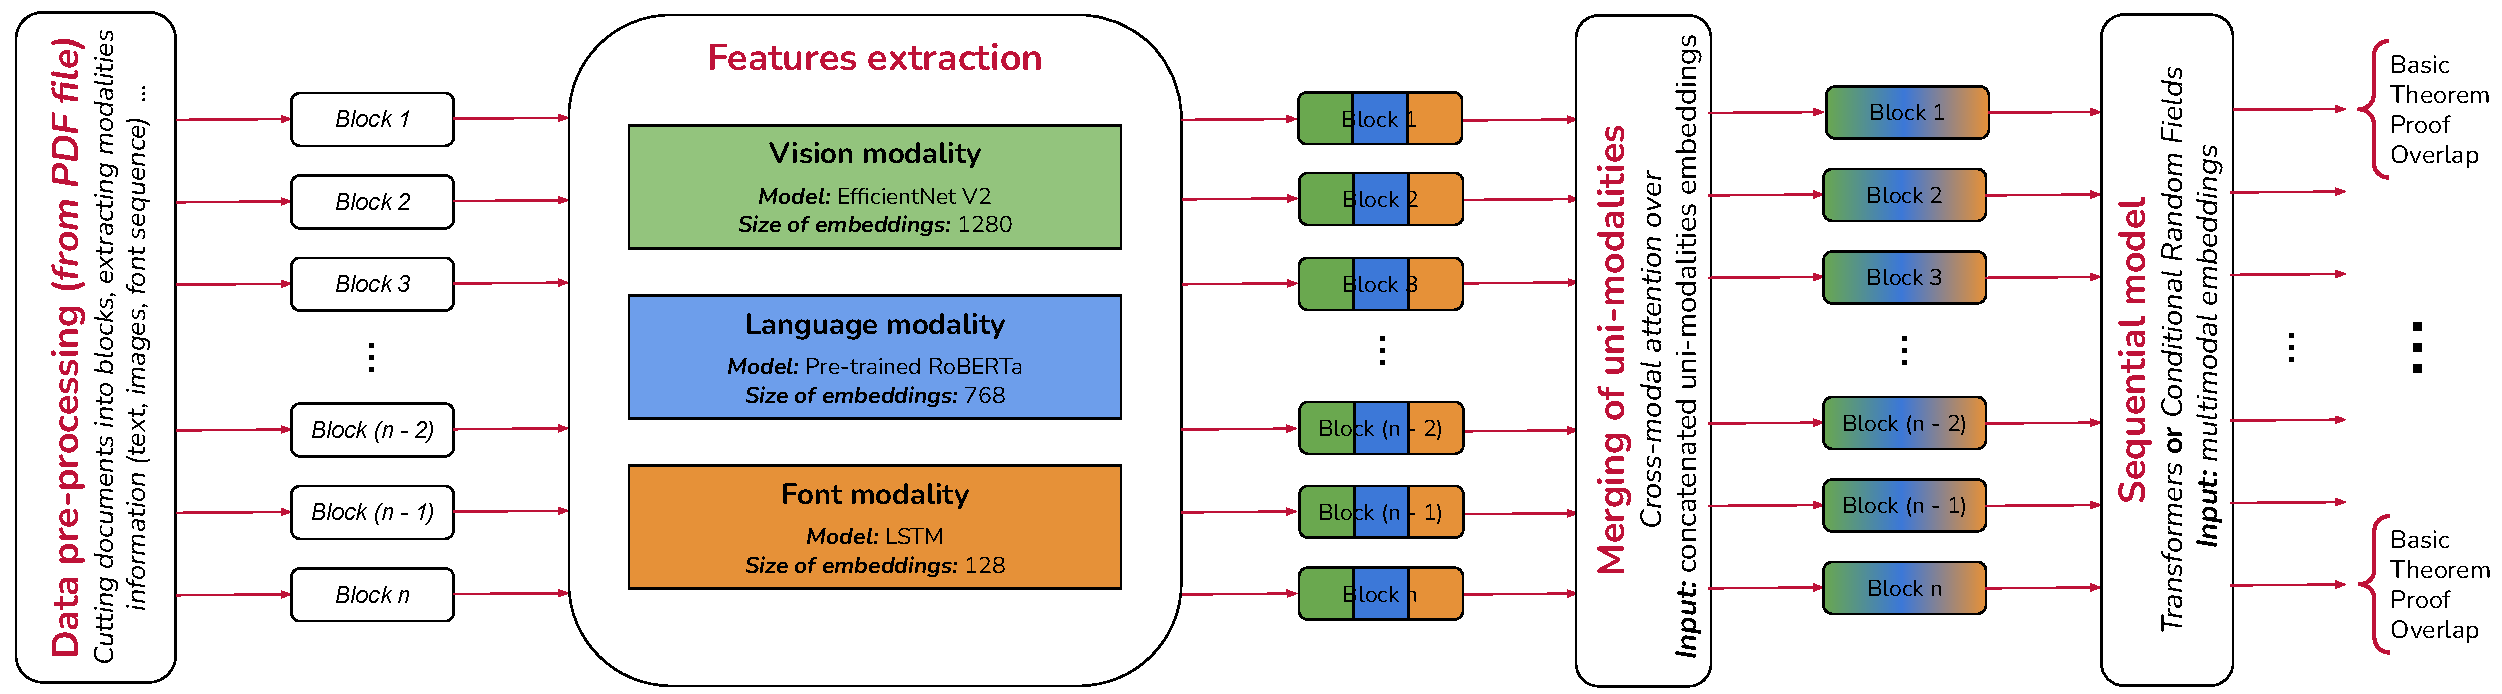
\includegraphics[width=\textwidth]{images/general_pipeline.pdf}
    \caption{Model inference from various modality (adding the sequential paragraph component)}
    \label{fig:generalpipeline}
\end{figure}


With a set of base features extracted from either the unimodal or multimodal approaches, we generate 
features for all paragraphs within the PDF. This process incorporates normalized page information, 
normalized coordinate data for each paragraph, and paragraph embeddings derived from the raw features 
just before the softmax layer. To capture sequential information across multiple paragraphs, we train a 
Conditional Random Field (CRF)~\cite{crf} or Transformer layer on top of the extracted features. The goal is to utilize 
relative information to contextualize each paragraph and accurately determine its label. Our model 
categorizes paragraphs into four major classes: (1) Proof-like, (2) Theorem-like, (3) Basic (neither 
proof nor theorem), and (4) an Overlap reject class that arises from preprocessing discrepancies.

\section{Demonstation scenario}

The UI of the demo is organized into several segments (for an overview see Figure~\ref{fig:system-arch}), each serving a specific function:

\begin{figure}[h]
    \centering
    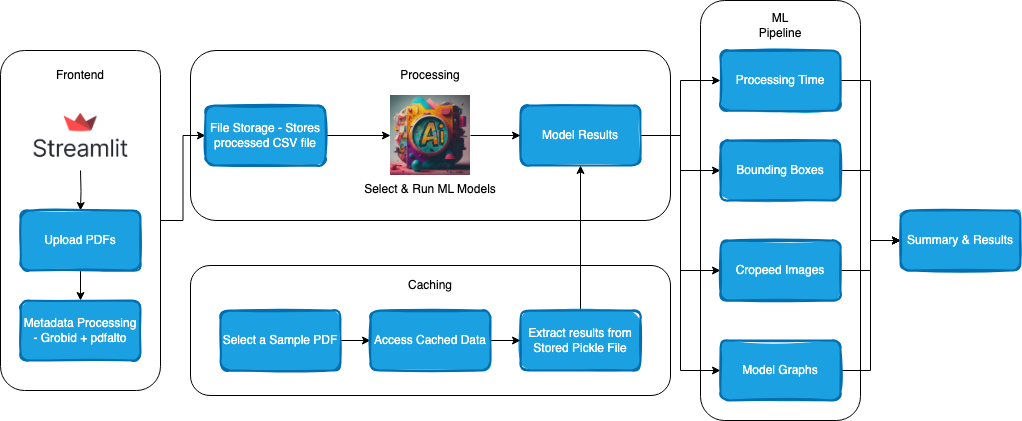
\includegraphics[width=\textwidth]{images/sys-demo-arch.png}
    \caption{Systems architecture of the various UI components
    }
    \label{fig:system-arch}
\end{figure}

The TheoremView demo interface is built using Streamlit and follows a modular architecture organized into distinct functional components. The frontend allows users to upload PDFs or select from cached samples, which then undergo metadata processing using Grobid and pdfalto tools. The processed data is stored as CSV files in the file storage component. The processing pipeline enables users to select and run various ML models (unimodal or multimodal) on the processed data. The ML pipeline component processes the data through multiple stages - calculating processing time, generating bounding boxes for visual elements, creating cropped images of detected theorems/proofs, and producing analytical graphs. These outputs are aggregated into comprehensive summary results. The system implements an efficient caching mechanism where frequently accessed PDFs and their corresponding ML model results are stored as pickle files, enabling instant retrieval without reprocessing. This architecture ensures smooth user interaction while maintaining high performance through optimized data flow and storage strategies.

\begin{enumerate}
    \item \textbf{Upload and Process}: Users can upload a PDF for processing or select from a list of previously 
    cached examples. The system processes the PDF by applying Grobid and pdfalto, converting each page into a bitmap image, 
    and merging the XML outputs from pdfalto and Grobid to generate a preprocessed \texttt{data.csv} file.

    \item \textbf{Predict and Preview}: Users can choose which base model to apply, either unimodal or multimodal, along with 
    sequential processing of paragraphs using a Conditional Random Field (CRF), Transformer, or no sequential processing at all, 
    allowing for a total of 12 possible combinations. Additionally, users have the option to preview or download the results 
    (see Figure~3 for visualization of results).

    \begin{figure}[h]
        \centering
        \begin{subfigure}{0.45\textwidth}
            \centering
            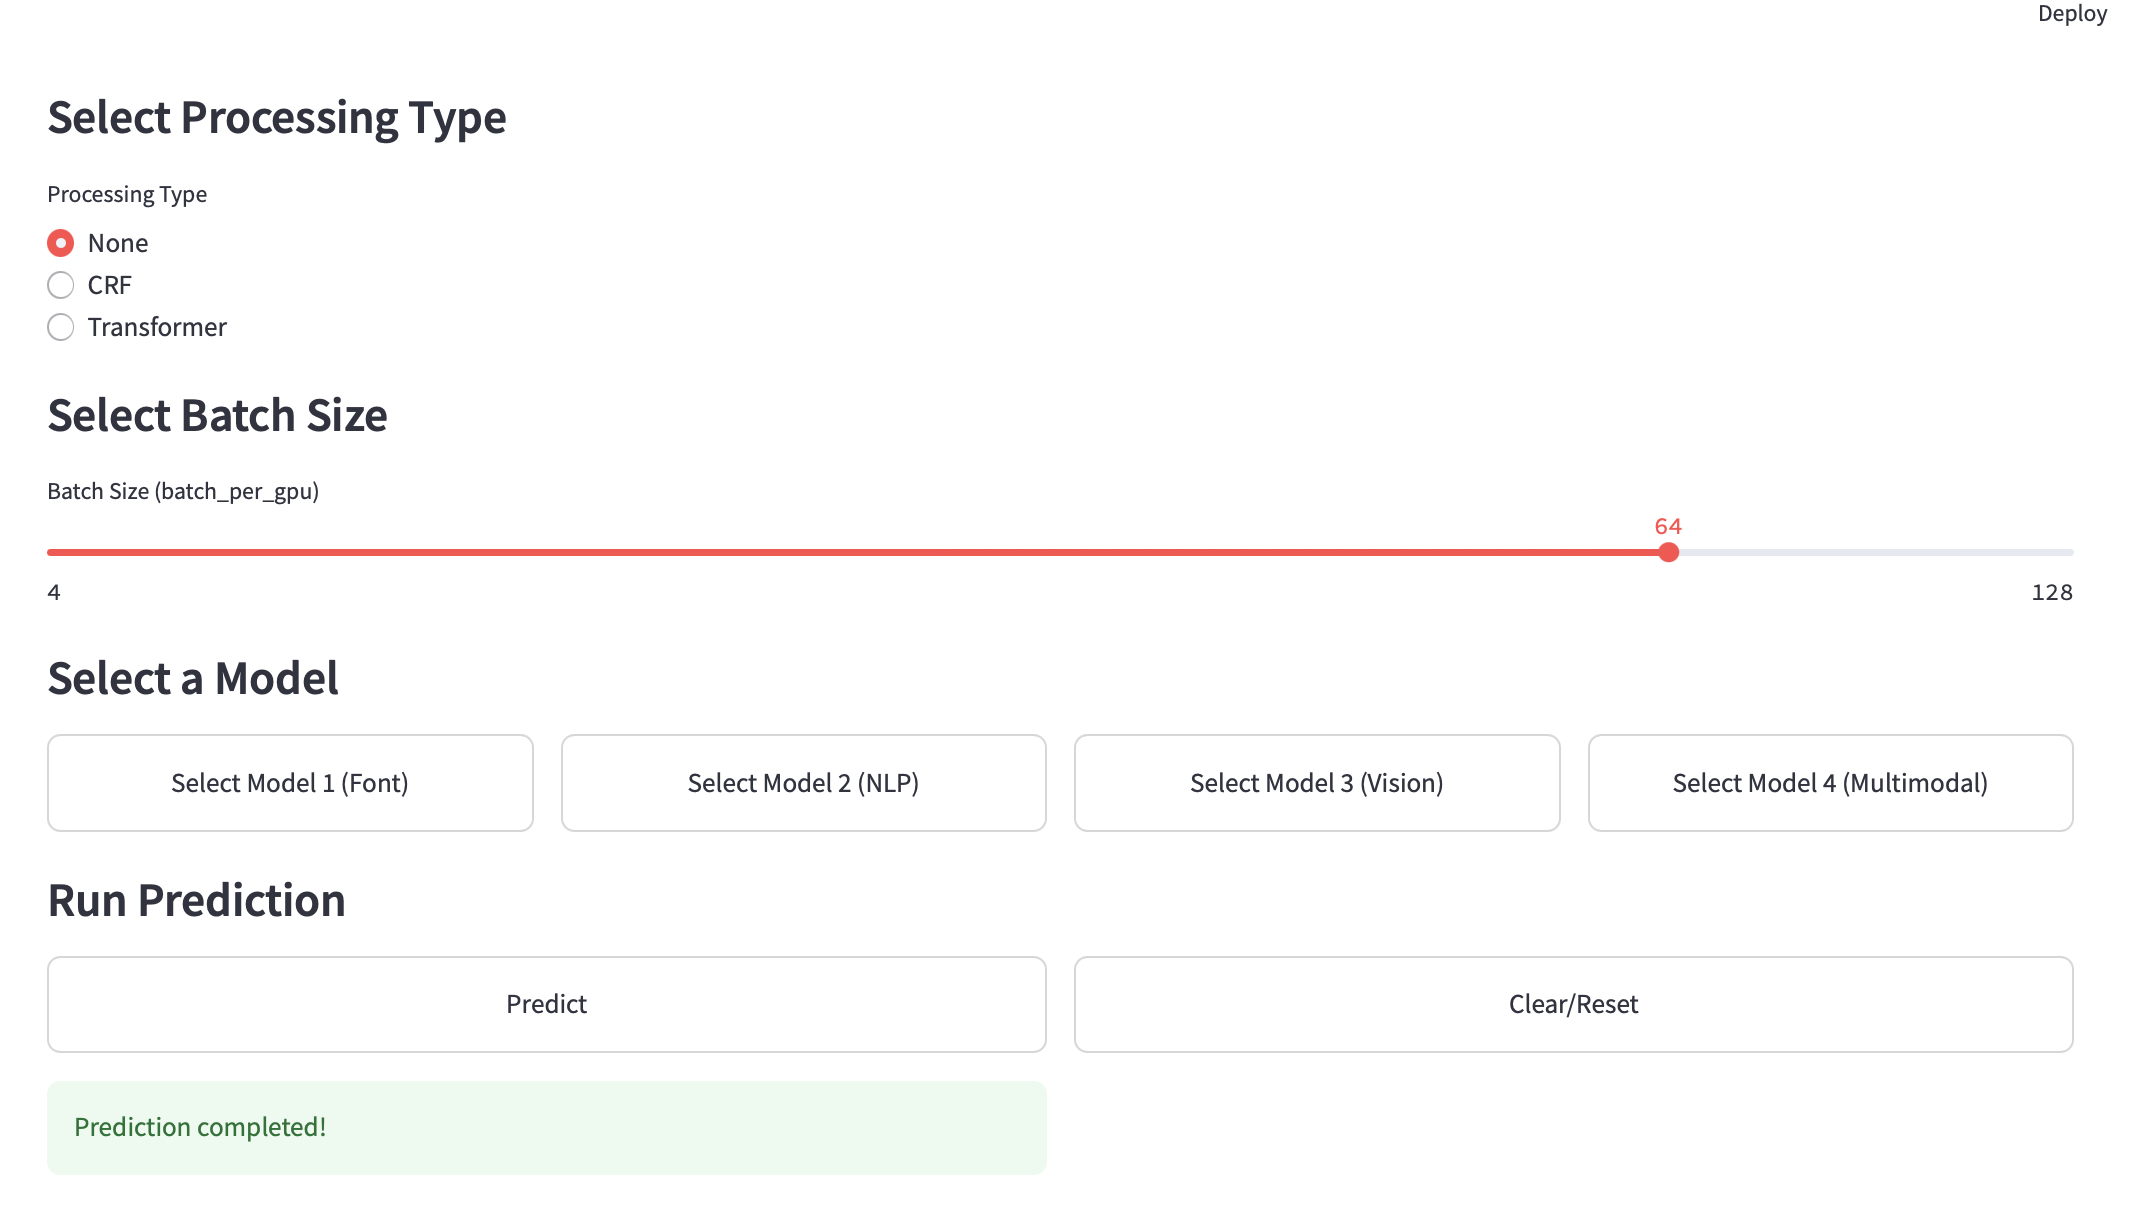
\includegraphics[width=\textwidth]{images/buttons.png}
            \caption{UI Buttons to run select the prediction model}
            \label{fig:buttons}
        \end{subfigure}
        \hfill
        \begin{subfigure}{0.45\textwidth}
            \centering
            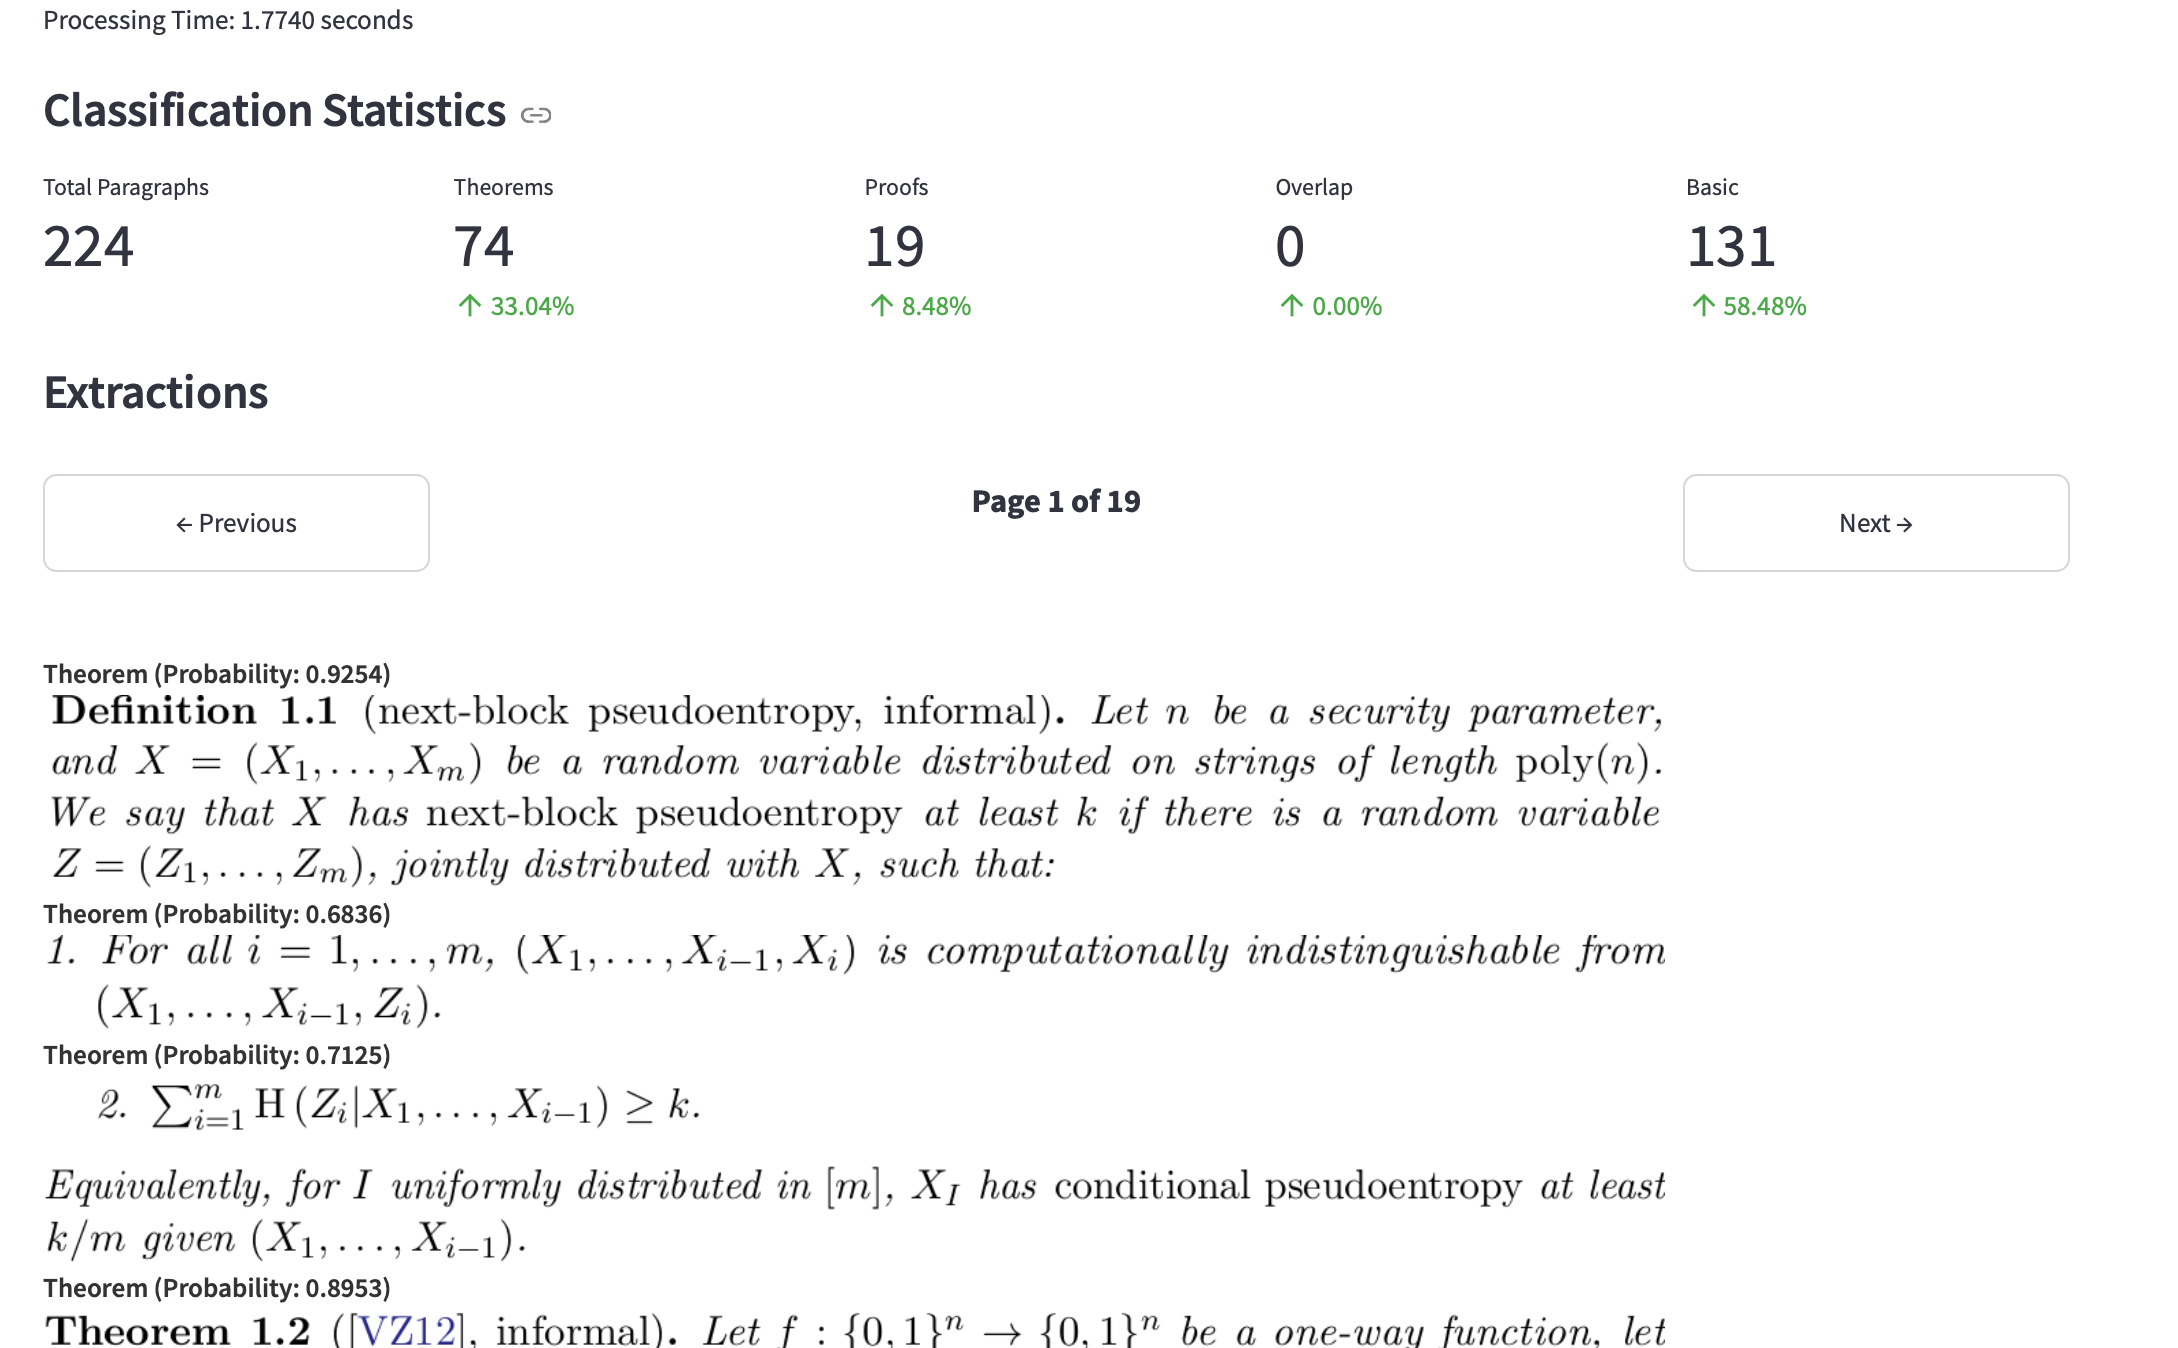
\includegraphics[width=\textwidth]{images/extractions.png}
            \caption{Extracted Information}
            \label{fig:extractions}
        \end{subfigure}
        \vskip\baselineskip
        \begin{subfigure}{0.45\textwidth}
            \centering
            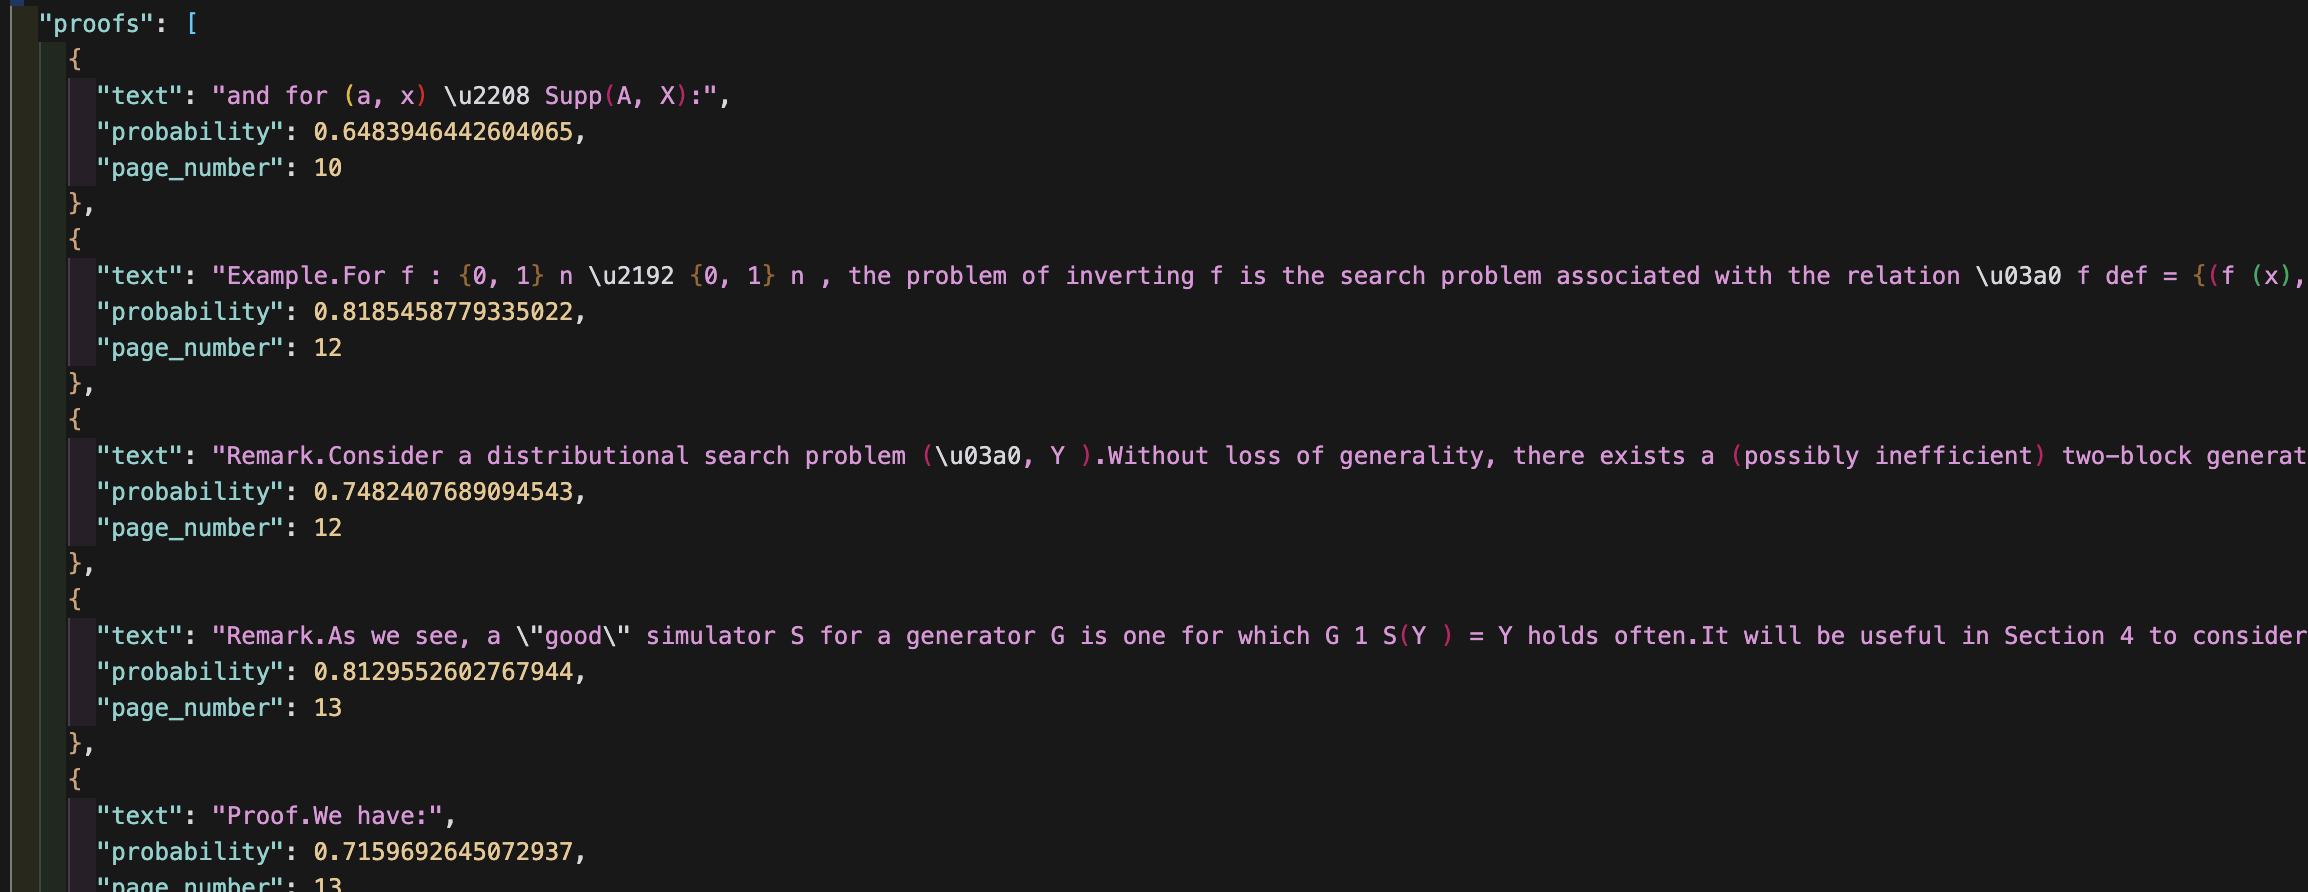
\includegraphics[width=\textwidth]{images/json_output.png}
            \caption{Extracted Information in JSON format.}
            \label{fig:json_output}
        \end{subfigure}
        \hfill
        \begin{subfigure}{0.45\textwidth}
            \centering
            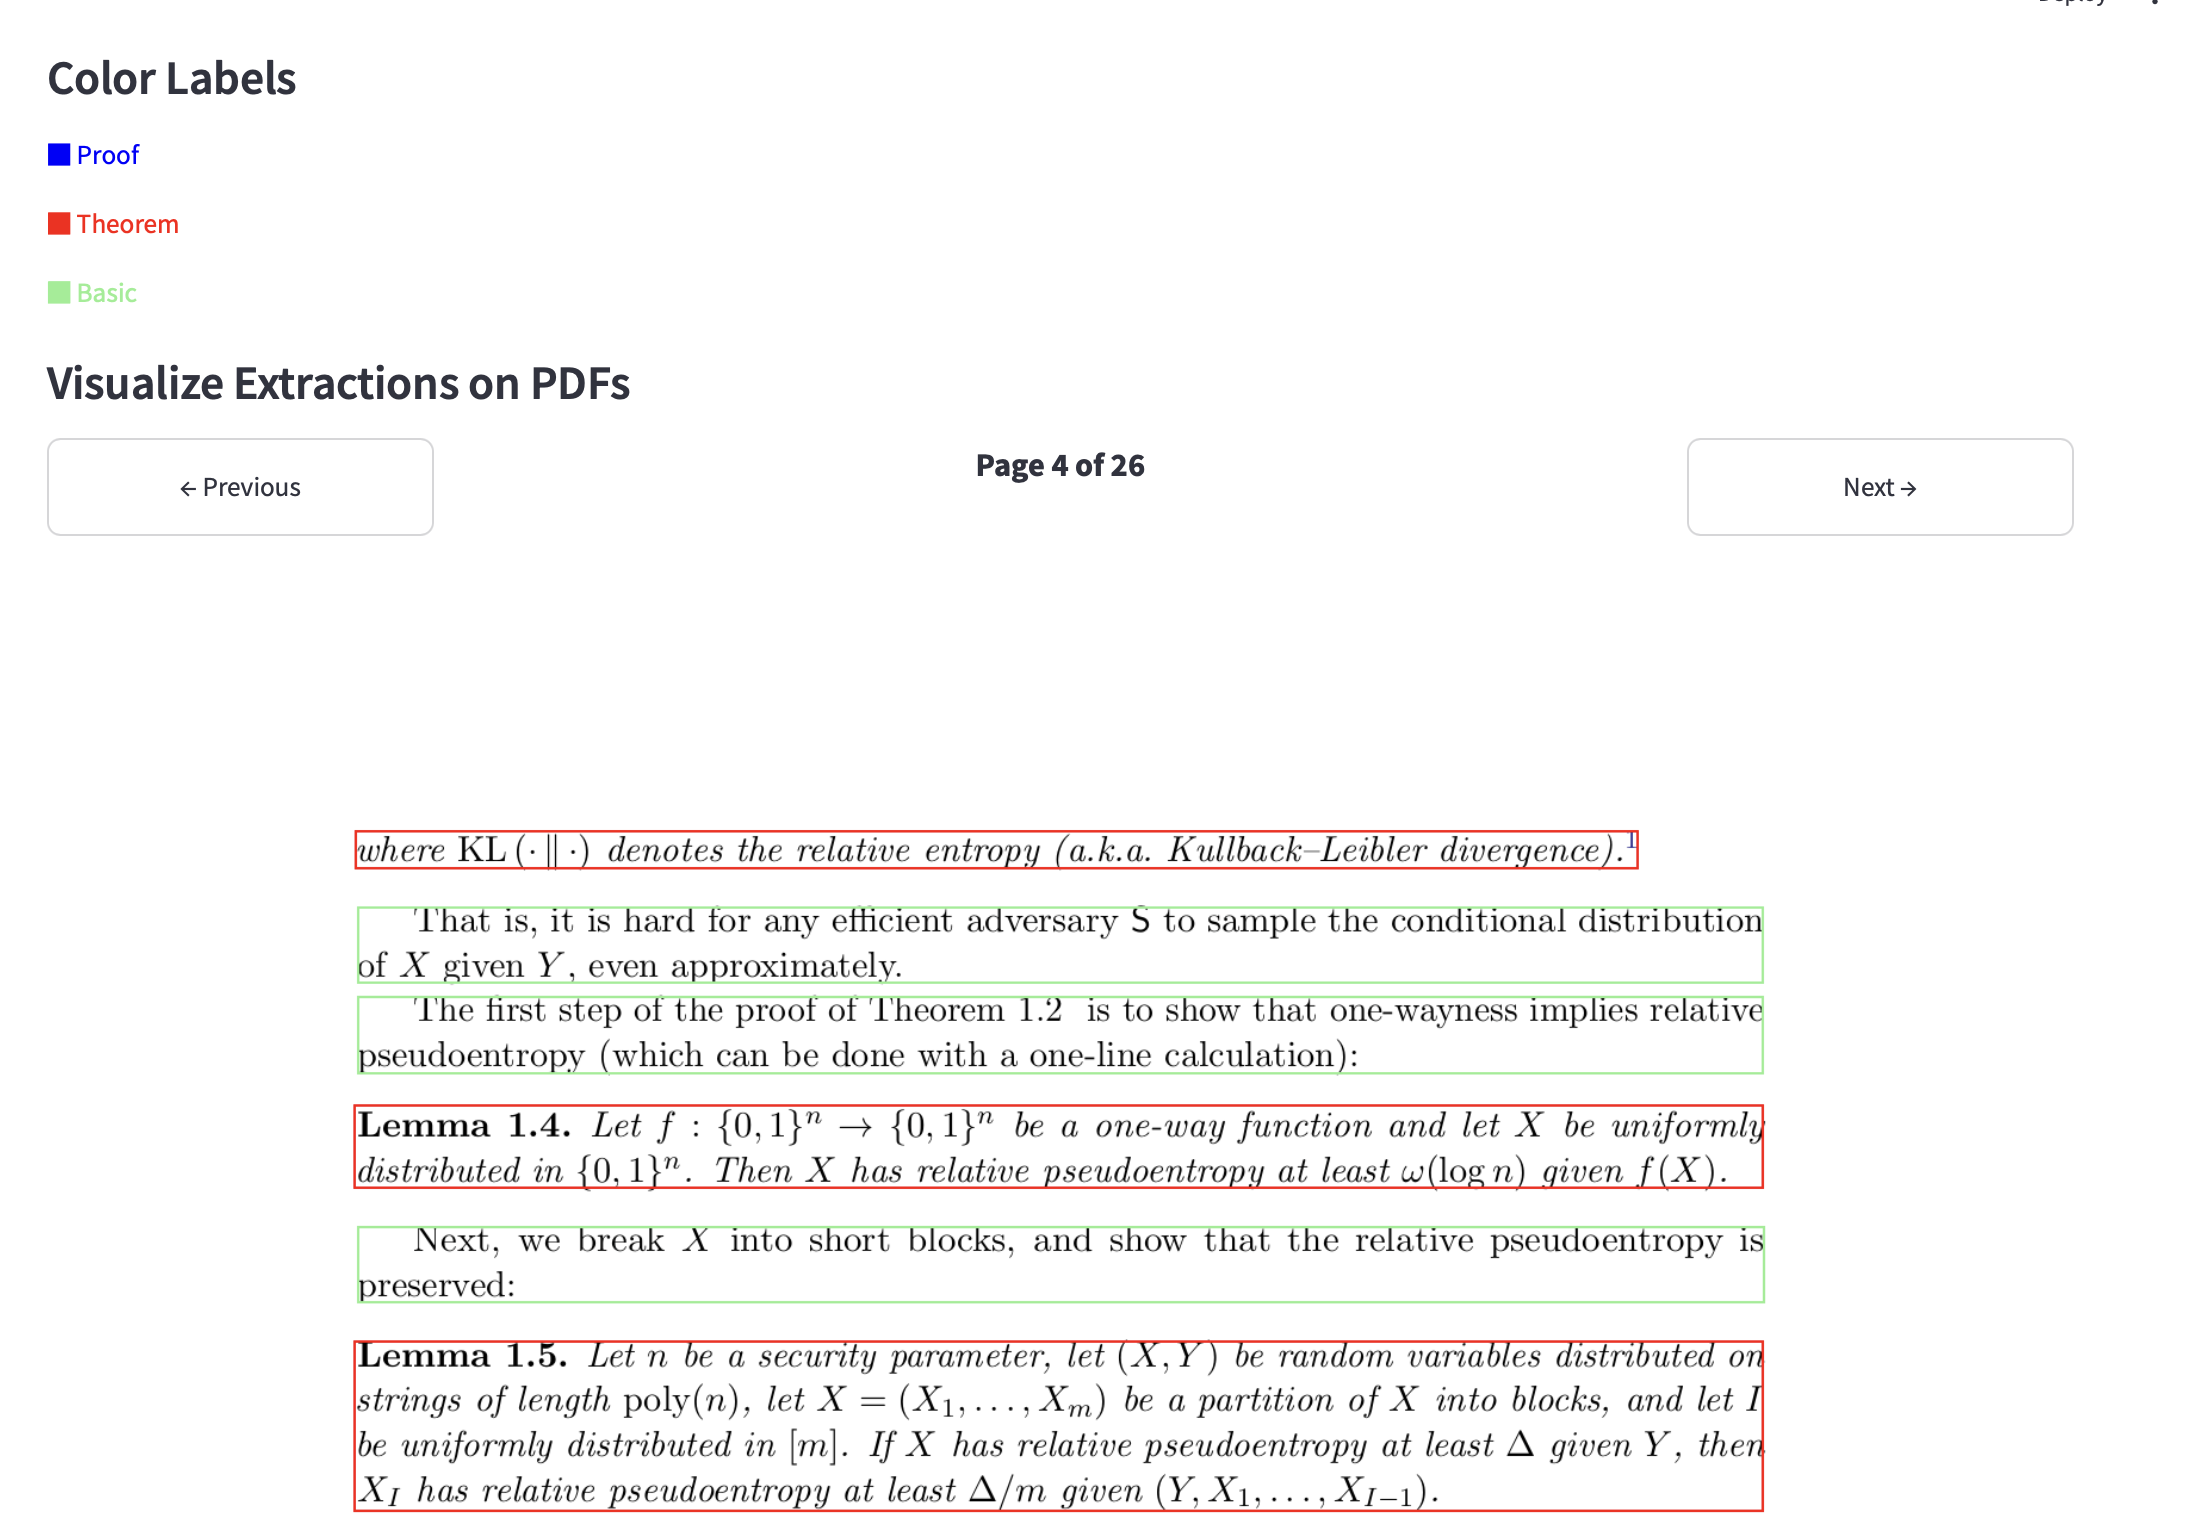
\includegraphics[width=\textwidth]{images/vis_on_pdf.png}
            \caption{Visualizations annotated on the PDF.}
            \label{fig:vis_on_pdf}
        \end{subfigure}
        \caption{Various visual elements in the demo.}
        \label{fig:combined}
    \end{figure}

    \item \textbf{Summary and Statistics}: This section provides a breakdown of the inference time for the current run, as well as 
    for any previous runs that have been cached, enabling comparative analysis (see Figure~\ref{fig:model_comp}).

    \begin{figure}[h]
        \centering
        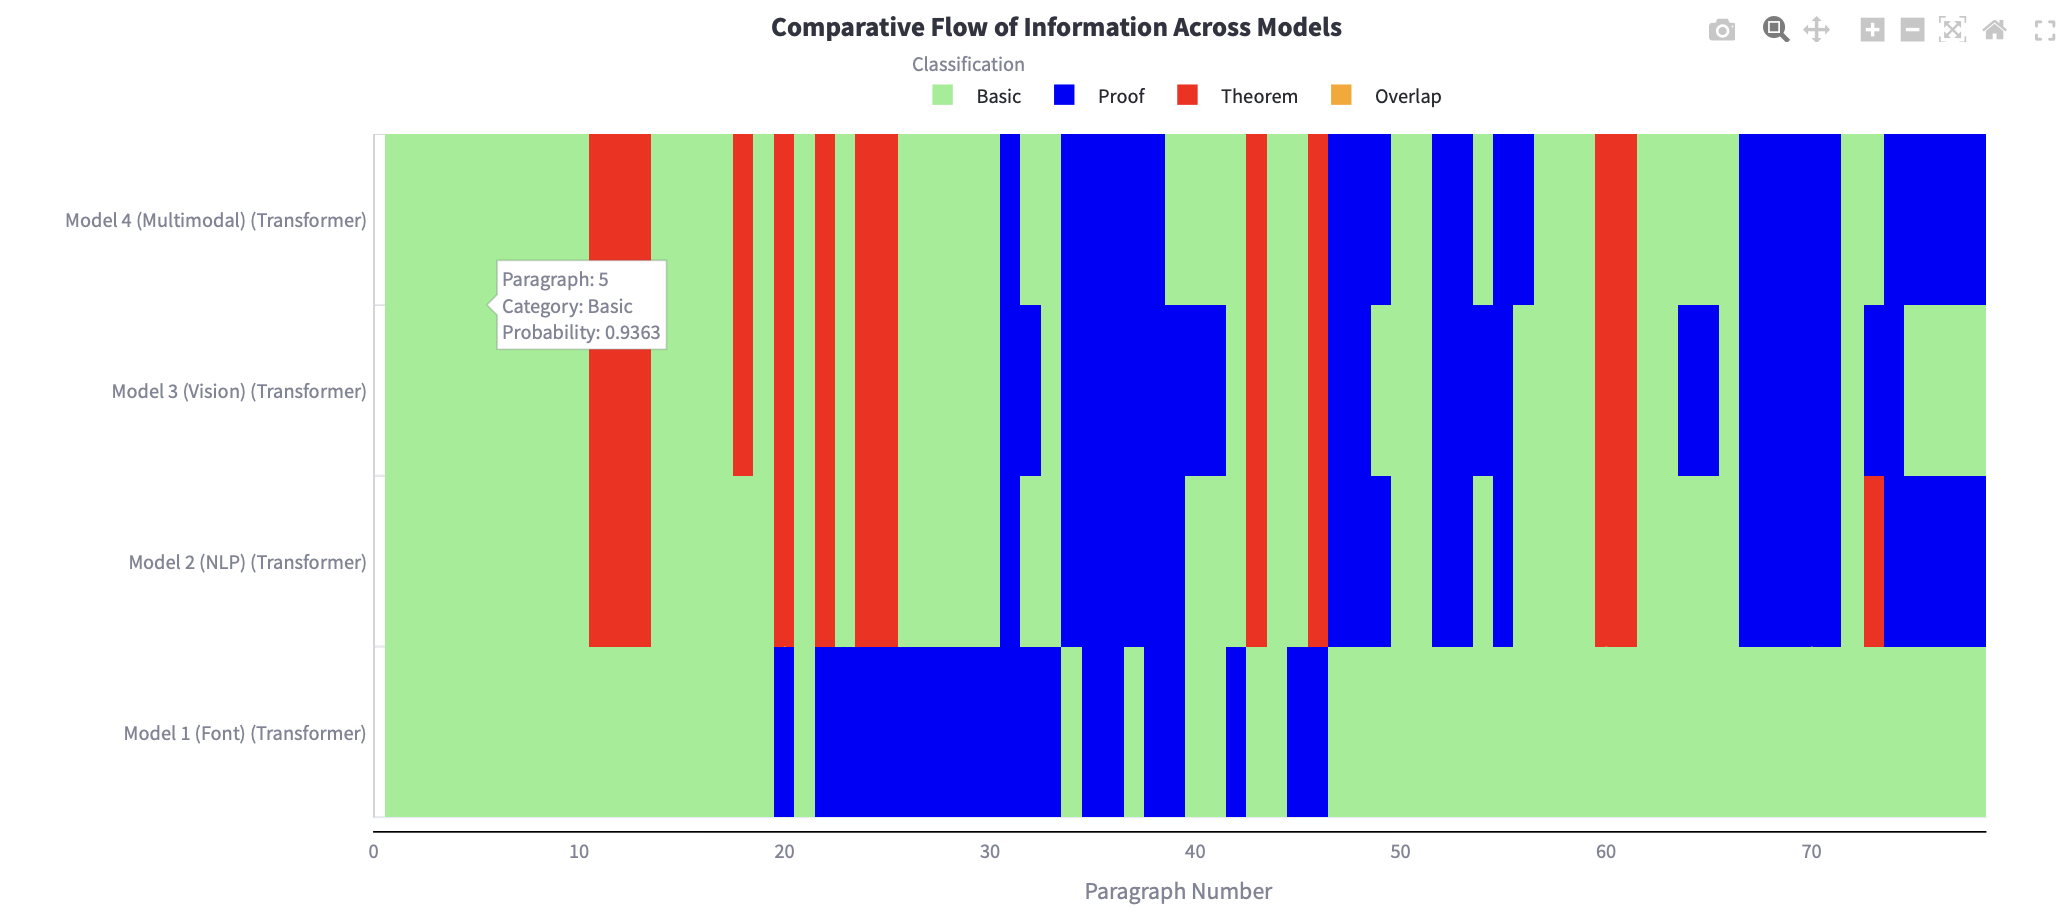
\includegraphics[width=\textwidth]{images/comparitive.png}
        \caption{Comparisons of predictions from different model runs}
        \label{fig:model_comp}
    \end{figure}
\end{enumerate}

%
\begin{thebibliography}{10}
\bibitem{doceng_paper}
Mishra, S., Pluvinage, L., Senellart, P.: Towards extraction of theorems and proofs in scholarly articles. In: Healy, P., Bilauca, M., Bonnici, A. (eds.) DocEng '21: ACM Symposium on Document Engineering 2021, Limerick, Ireland, August 24-27, 2021, pp. 25:1--25:4. Association for Computing Machinery, New York, NY, USA (2021). \doi{10.1145/3469096.3475059}

\bibitem{mishra2024first}
Mishra, S., Brihmouche, Y., Delemazure, T., Gauquier, A., Senellart, P.: First steps in building a knowledge base of mathematical results. In: Proceedings of the Fourth Workshop on Scholarly Document Processing (SDP 2024), pp. 165--174 (2024)

\bibitem{jcdl_paper}
Mishra, S., Gauquier, A., Senellart, P.: Multimodal Machine Learning for Extraction of Theorems and Proofs in the Scientific Literature. CoRR abs/2307.09047 (2023). \doi{10.48550/arXiv.2307.09047}

\bibitem{hochreiter1997long}
Hochreiter, S., Schmidhuber, J.:  Long short-term memory. In: Neural computation 9, 8 (1997)

\bibitem{arevalo2020gated}
Arevalo, J., Solorio, T., Montes-y Gómez, M., A González, F.: Gated multimodal networks. In: Neural Computing and Applications 32 (2020). 

\bibitem{GROBID}
GROBID: \url{https://github.com/kermitt2/grobid}, GitHub (2008--2024). swh:1:dir:dab86b296e3c3216e2241968f0d63b68e8209d3c

\bibitem{pdfalto}
pdfalto: \url{https://github.com/kermitt2/pdfalto}, GitHub (2017--2024). swh:1:dir:4b5e8b8c8e3c3216e2241968f0d63b68e8209d3c

\bibitem{efficientnet}
Tan, M., Le, Q.V.: EfficientNetV2: Smaller Models and Faster Training. In: Proceedings of the 38th International Conference on Machine Learning, PMLR 139, pp. 10096--10106 (2021)

\bibitem{crf}
Lafferty, J., McCallum, A., Pereira, F.C.N.: Conditional Random Fields: Probabilistic Models for Segmenting and Labeling Sequence Data. In: Proceedings of the Eighteenth International Conference on Machine Learning, ICML '01, pp. 282--289. Morgan Kaufmann Publishers Inc., San Francisco, CA, USA (2001)

\bibitem{transformer}
Vaswani, A., Shazeer, N., Parmar, N., Uszkoreit, J., Jones, L., Gomez, A.N., Kaiser, Ł., Polosukhin, I.: Attention is All you Need. In: Advances in Neural Information Processing Systems, pp. 5998--6008 (2017)
\end{thebibliography}
\end{document}
